\documentclass[../thesis.tex]{subfiles}
 
\begin{document}
 
 
% Deep IRL in off-road environment
 
Most of the robotics problems can be solved under optimization framework.
For the motion planning problem, the objective is to find a sequence of control actions that minimizes the accumulated costs toward the goal state.
Reinforcement learning, on the other hand, formulates the problem as finding a policy that maximizes the expected accumulated rewards collected from the environment.
Both problems require a definition of the cost/reward function of the interested robotics tasks.
However, unlike in the urban environment where cost function can be well defined in a rule-based structure, finding a cost function for off-road navigation can be non-trivial and often requires lots of handy tunings \cite{silver2010learning}.
Here, motivated by the recent successes \cite{wulfmeier2015maximum,wulfmeier2016watch} to using deep neural nets to approximate the cost functions, we implement a similar algorithm for the off-road application.
 
 
\section{Proposed Methods}
 
\begin{figure}[t]
        \begin{center}
         \centerline{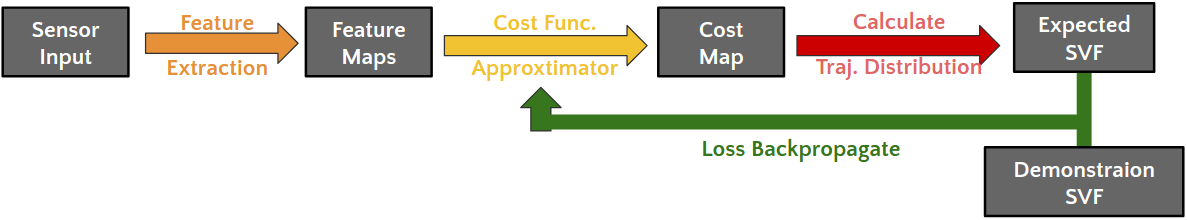
\includegraphics[width=\columnwidth]{./DIRL/fig/dirl_diagram.png}}
               \caption{Block diagram of deep inverse reinforcement learning.}
               \label{fig:dirl_diagram}
        \end{center}
        \vskip -0.2in
\end{figure}
 
The pipeline of deep inverse reinforcement learning (DIRL) is shown in Fig. \ref{fig:dirl_diagram}.
The raw sensor inputs first process through the feature extraction module.
The resulting feature maps are used as the input of the cost function that is approximated by a deep neural network.
Once the cost map is generated, we can formulate the corresponding Markov Decision Process (MDP) problem and solve for the expected state-visited frequencies (SVF).
Finally, the gradient is applied using Eq. \ref{equ:dirl_grad} by comparing the expected SVF inferred under the current reward structure with the target SVF calculated from the demonstrations.
 
\subsection{Learning from Failure for DIRL}
 
%%% Challenge %%%
The fundamental challenge arises with DIRL is the spatially sparse gradient feedback.
Since the gradient signals only come from the difference between demonstrations and expected trajectories, the loss feedbacks in training will inevitably focus more on the traversable regions.
The problem can be alleviated by pre-training the network under standard image segmentation framework \cite{wulfmeier2016incorporating}, which provide pixel-wise feedbacks for error terms.
Here, we propose an alternative approach that re-formulated the same problem with \textit{negative} demonstrations.
 
Following the same convention in Section \ref{sec:dirl_intro}, we now denote the positive and negative demonstrations as $D_{pos}$ and $D_{neg}$, respectively. The log likelihood (Eq. \ref{equ:dirl_obj}) can be reformulated as:
 
\begin{align}
L(\theta) &= \log P(D_{pos}, D_{neg},\theta|r) \\
&= \log P(D_{pos}|r) + \log P(D_{neg}|r^{-1}) + \log P(\theta)
\end{align}
 
With the L2-regularization, the new gradient becomes:
 
\begin{align}
\frac{\partial L}{\partial \theta} &= \left( \mu_{D_{pos}} - \mathbb{E}_{r}[\mu] \right) \frac{\partial r}{\partial \theta} + \left( \mu_{D_{neg}} - \mathbb{E}_{r^{-1}}[\mu] \right) \frac{\partial r^{-1}}{\partial r} \frac{\partial r}{\partial \theta} + \frac{\lambda}{2} \| \theta \|^2 \\
&= \left( \mu_{D_{pos}} - \mathbb{E}_{r}[\mu] + \mathbb{E}_{r^{-1}}[\mu] - \mu_{D_{neg}} \right) \cdot \frac{\partial r}{\partial \theta} + \frac{\lambda}{2} \| \theta \|^2
\end{align}
 
where $r^{-1} = constant - r $ stands for the \textit{inverted} reward map.
By jointly optimizing with the negative demonstrations, we can increase the gradient feedbacks for non-traversable regions where the positive demonstrations will never capture.
 
\subsection{Modeling Optimality Ambiguity}
 
As described in Section \ref{sec:dirl_intro}, the objective function of IRL is usually formulated either in a fashion of structured support vector machines (SSVMs), or conditional random fields (CRFs).
While Maximum Margin Planning (MMP) falls in the first category, Maximum Entropy IRL (ME-IRL) can represent the second category.
However, both categories share a similar form of the gradient of its objective.
Recall Eq. \ref{equ:mmp_obj} and Eq. \ref{equ:dirl_grad}, while gradient of MMP involves in solving the \textit{optimal} trajectory on the evolving reward map, the gradient of ME-IRL instead requires solving the \textit{expectation} of the trajectory distribution.
The rest calculations remain mostly the same.
\citet{pletscher2010entropy} proposed a generalized loss that models the observed expert behaviors with Gibbs distribution and an inverse temperature $\beta \in \mathbb R^{+}$.
 
\begin{align}
P_{\beta}(\xi_i | r_\theta) &= \frac{1}{Z_\beta} \exp \left( \beta r_\theta(\xi_i) \right) \\
\text{,where \quad} Z_\beta &= \sum_{\xi \in \Xi} \exp \left( \beta r_\theta(\xi) \right) \text{is the normalization constant.}
\end{align}
 
As $\beta$ increases, the exponent term dominates, and the corresponding distribution becomes sharper.
If $\beta \to \infty$, the distribution degenerates to solving the $\arg\max$, \textit{i.e.} the optimal trajectory 
$P(\xi_i | r_\theta)= \mathbbm{1}\left\{ \xi_i = \argmaxE_{\xi \in \Xi} r_\theta(\xi) \right\}  $.
On the other hand, if $\beta \to 1$, the distribution becomes the same form of the one used in ME-IRL.
In other words, the SSVM-like and CRF-like losses are framed under the same framework and can be seen as two special cases located at the opposite side of the spectrum.
$\beta \to 0 P(\xi_i | r_\theta)= uniform $


This generalized loss introduces a new parameter $\beta$ that captures on which level of the \textit{optimality} is presented by the demonstration trajectories. By integrating this generalized loss in our computational graph, the parameter can be optimized jointly during training.
 
\section{Experiments Results}
 
\begin{figure}[t]
        \begin{center}
         \centerline{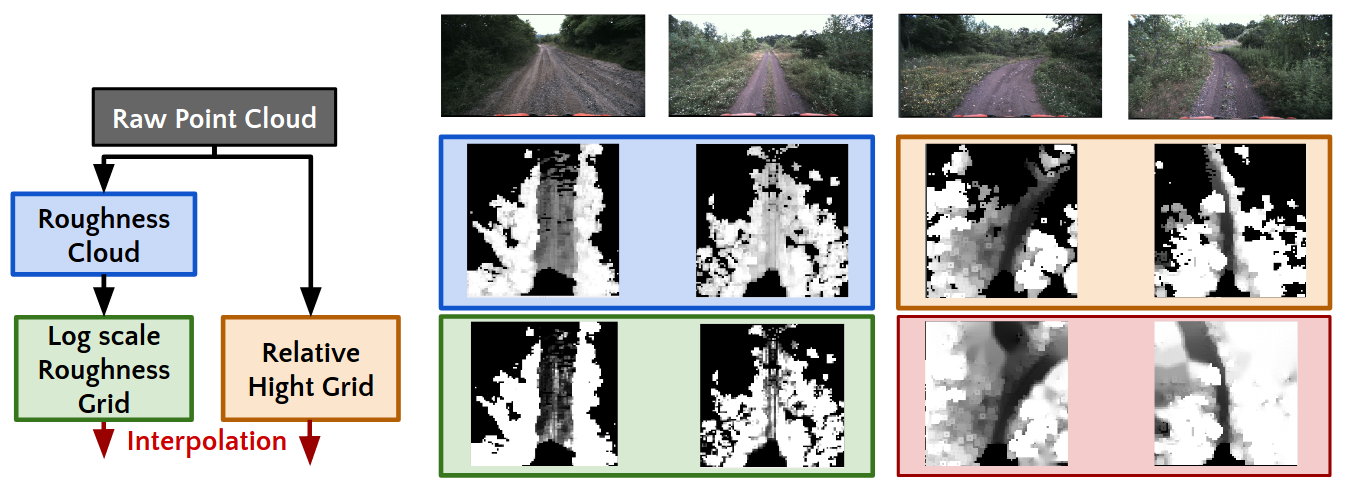
\includegraphics[width=\columnwidth]{./DIRL/fig/lidar_feature_map.png}}
               \caption{The extracted feature maps from LiDAR. The flow chart is shown on the left of the figure, while examples of the actual collected data on field are shown on the right of the figure.}
               \label{fig:lidar_feature_map}
        \end{center}
        \vskip -0.2in
\end{figure}
 
 
\begin{figure}[t]
        \begin{center}
         \centerline{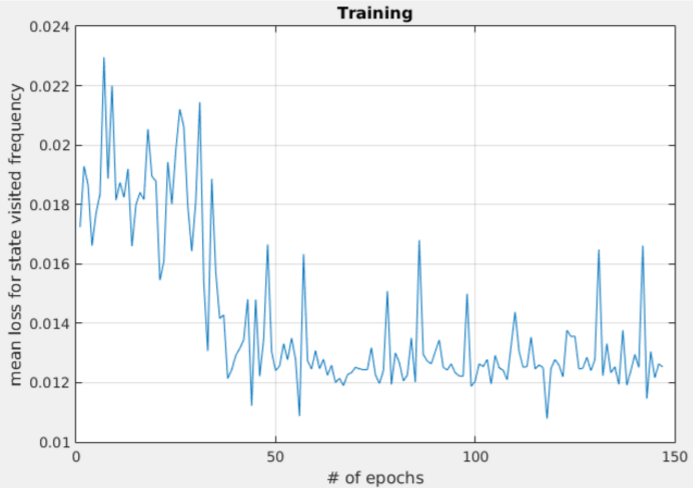
\includegraphics[width=0.5\columnwidth]{./DIRL/fig/dirl_training_curve.png}}
               \caption{Training curve of DIRL in Gascola dataset.}
               \label{fig:dirl_learning_curve}
        \end{center}
        \vskip -0.2in
\end{figure}
  
\begin{figure}[t]
        \begin{center}
         \centerline{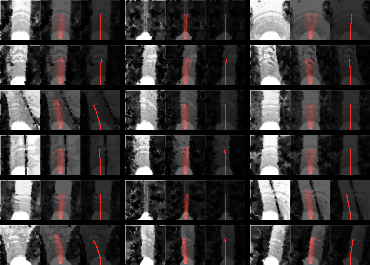
\includegraphics[width=0.8\columnwidth]{./DIRL/fig/gradtestImg040.png}}
               \caption{Final cost map on testing set. The left, middle, and right image represent the output cost map, the same cost map overlapped with expected SVF, and with demonstrations, respectively.}
               \label{fig:final_cost_map}
        \end{center}
        \vskip -0.2in
\end{figure}
 
\begin{figure}[t]
      \begin{center}
       \centerline{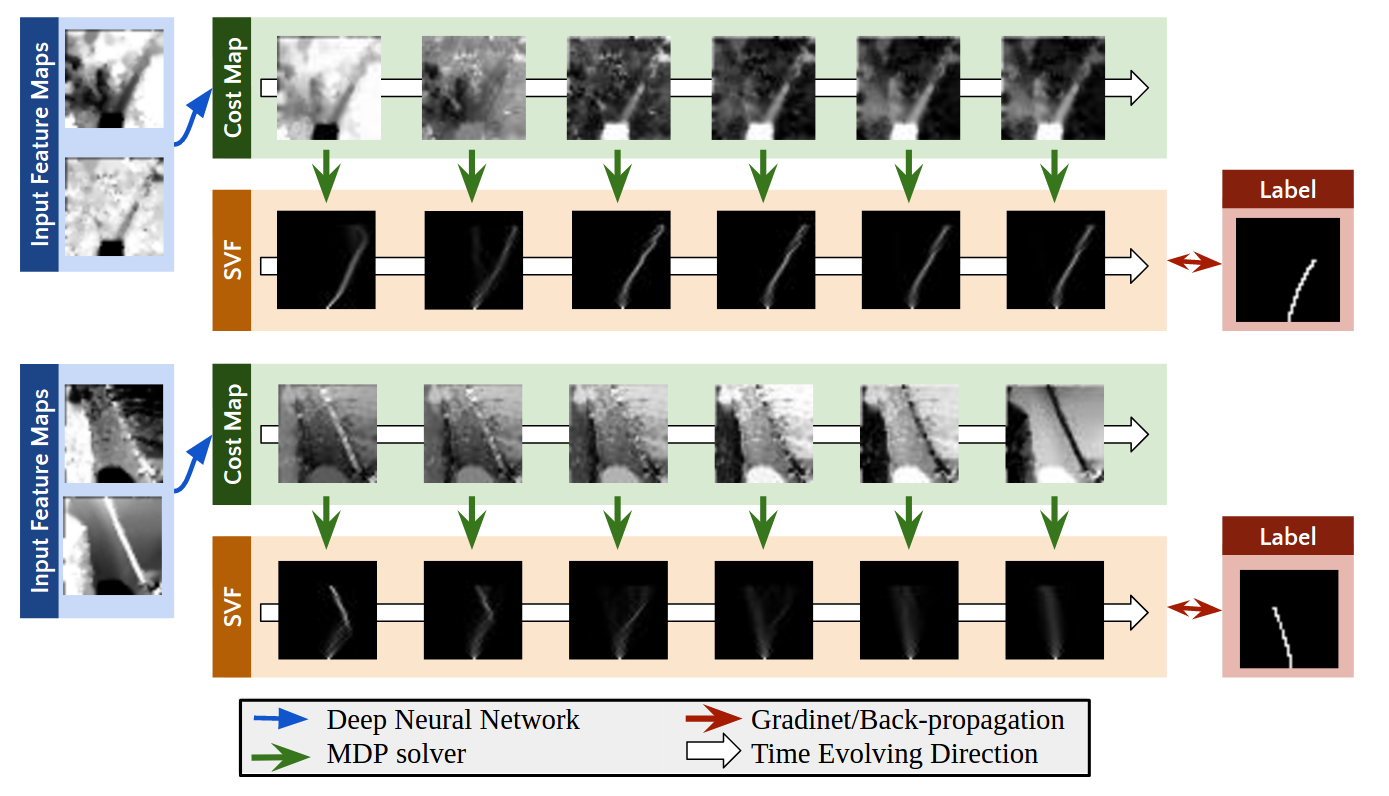
\includegraphics[width=\columnwidth]{./DIRL/fig/inter_cost_map.png}}
            \caption{Samples of intermediate cost maps during training.}
            \label{fig:inter_cost_map}
      \end{center}
      \vskip -0.2in
\end{figure}

Following the similar setup in Chapter \ref{chap:rrtplanner}, we use Yamaha Viking VI side-by-side ATV as our main testing platform, with LiDAR as our primary input sensor.
For off-road navigation where scenes can change dramatically, LiDAR provides a more reliable measurement for the safety concern.
In addition, informative features such as terrain roughness can be inferred straight-forwardly.
We collect the dataset with total 150 human demonstrations covering an off-road testing field at Gascola, PA. Each sample covers the $20m \times 20m$ region in the front of the ATV. Since the Gascola dataset is relatively small, we use a shallow multilayer perception as the cost function.
 
The first feature map captures information about terrain roughness.
As shown in Fig. \ref{fig:lidar_feature_map}, the basic approach to infer terrain roughness from the raw point cloud is to first divide it into patches.
For each patch, a normal plane is fitted using standard least square regression.
Once the plane parameters are calculated, the \textit{roughness index} can be inferred by averaging plane variances within each patch.
However, this naive roughness index is sensitive to hyper-parameter such as patch size and rescaling factors.
In off-road environments where terrain types can vary a lot, this approach can fail to extract reasonable features when trails become narrow, as shown in the second column of Fig. \ref{fig:lidar_feature_map}.
To alleviate this issue, we replace the original roughness index with the log-scale value.
The log scale helps amplify the slight difference among traversable terrains in which we have more interests.
On the other hand, the roughness difference among the non-traversable terrain such as bush or trees is flattened under the log scale.
Another informative feature map is the relative height with respect to the vehicle standing level.
 
 
The intuition behind the two feature maps is that the vehicle should prefer driving over terrain that is smoother or at the similar horizontal level of its current local frame.
Note that both feature maps are projected on a top-down view, leaving some parts of the feature maps unoccupied.
However, the invisible grids may confuse the network and make the framework fragile to the senses.
Though the problem can be alleviated by simply providing an additional feature map that specifies the visibility, it usually requires much more data and the use of convolution layer \cite{wulfmeier2015maximum,wulfmeier2016watch}.
Since our dataset is relatively small, we alleviate this issue with an alternative approach.
Instead, we apply a standard image inpainting technique \cite{telea2004image} that effectively helps infer the invisible region given the geometric shape of the visible trails.
The feature maps before and after the interpolation are shown in the orange and red area in Fig. \ref{fig:lidar_feature_map}, respectively.
 
The training curve is summarized in Fig. \ref{fig:dirl_learning_curve}, with the resulting cost maps on testing data set shown in Fig. \ref{fig:final_cost_map}. 
The training curve converges within $55$ episodes in our Gascola data set, yet the testing result shows its efficacy by capturing untraversable region like fences and distinguishing the nuance of terrain roughness on both wide and narrow trails.
Fig. \ref{fig:inter_cost_map} visualizes the intermediate cost maps of two samples during training, with the first and second row represent the intersection of a narrow trail, and a wider trail beside a fence, respectively.

\end{document}
